\documentclass[tikz,border=2pt]{standalone}
\usepackage{amsmath,amssymb}
\usetikzlibrary{arrows.meta,decorations.pathreplacing}
\begin{document}
% The same outage of length R placed two ways: non-preemptive (top), it starts only after job 2
% has finished; preemptive (bottom), it interrupts job 2, whose time at the server then contains
% its net service time plus the outage.
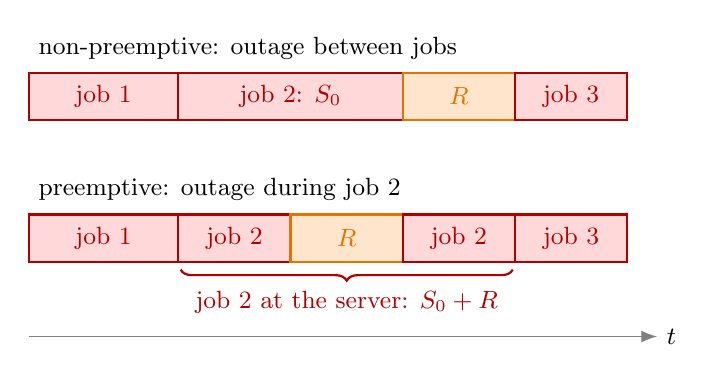
\begin{tikzpicture}[font=\small, >={Latex[length=2mm]}, x=0.95cm, y=1cm]
  \tikzset{job/.style={draw=red!70!black, fill=red!15, thick},
           outage/.style={draw=orange!90!black, fill=orange!20, thick}}
  % top row
  \node[anchor=south west] at (0,2.45) {non-preemptive: outage between jobs};
  \draw[job] (0,1.8) rectangle (2,2.4);   \node[red!70!black] at (1,2.1) {job 1};
  \draw[job] (2,1.8) rectangle (5,2.4);   \node[red!70!black] at (3.5,2.1) {job 2: $S_0$};
  \draw[outage] (5,1.8) rectangle (6.5,2.4); \node[orange!90!black] at (5.75,2.1) {$R$};
  \draw[job] (6.5,1.8) rectangle (8,2.4); \node[red!70!black] at (7.25,2.1) {job 3};
  % bottom row
  \node[anchor=south west] at (0,0.65) {preemptive: outage during job 2};
  \draw[job] (0,0) rectangle (2,0.6);     \node[red!70!black] at (1,0.3) {job 1};
  \draw[job] (2,0) rectangle (3.5,0.6);   \node[red!70!black] at (2.75,0.3) {job 2};
  \draw[outage] (3.5,0) rectangle (5,0.6);   \node[orange!90!black] at (4.25,0.3) {$R$};
  \draw[job] (5,0) rectangle (6.5,0.6);   \node[red!70!black] at (5.75,0.3) {job 2};
  \draw[job] (6.5,0) rectangle (8,0.6);   \node[red!70!black] at (7.25,0.3) {job 3};
  % brace: time job 2 occupies the server
  \draw[decorate, decoration={brace, amplitude=4pt, mirror}, red!70!black, thick] (2.03,-0.1) -- (6.47,-0.1)
    node[midway, below=4pt] {job 2 at the server: $S_0+R$};
  % time axis
  \draw[->, gray] (0,-0.95) -- (8.4,-0.95) node[right, black] {$t$};
\end{tikzpicture}
\end{document}
